\documentclass{standalone}
\usepackage{tikz}
\usepackage{ctex,siunitx}
\setCJKmainfont{Noto Serif CJK SC}
\usepackage{tkz-euclide}
\usepackage{amsmath}
\usetikzlibrary{patterns, calc}
\usetikzlibrary {decorations.pathmorphing, decorations.pathreplacing, decorations.shapes,}

\begin{document}
\small
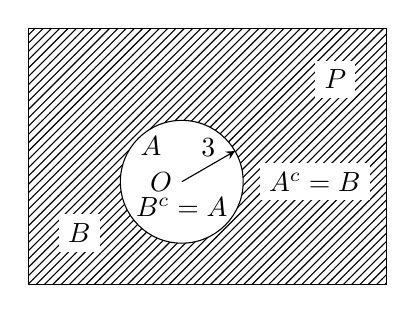
\begin{tikzpicture}[>=stealth,scale=1.3]
  \tkzSetUpPoint[fill=black]
  % \useasboundingbox(-1,-0.75)rectangle(3.7,1.4);
  \fill[pattern=north east lines, draw](0,0) rectangle (3.5,2.5);
  \draw [fill=white](1.5,1)node[left]{$O$} circle (.6);
  \node at (1.5,.75){$B^c=A$};
  \draw [->](1.5,1)--node[above]{3}+(30:.6);
  \node at (1.2,1.35){$A$};
  \node at (3,2)[fill=white]{$P$};
  \node at (2.8,1)[fill=white]{$A^c=B$};
  \node at (.5,.5)[fill=white]{$B$};
\end{tikzpicture}
\end{document}